\documentclass[11pt]{article}

%4pp das transps
% psnup -W415 -H273 -s.9 -b10 -d10 -c -4 05-Tecnicas_Compressao_Imagens.ps 05-Tecnicas_Compressao_Imagens.4pp.ps

\usepackage[utf8]{inputenc} % PARA USAR PALAVRAS EM PORT
%\usepackage[portuguese]{babel}
\usepackage{a4wide}
\usepackage{color}
\usepackage{colordvi}
\usepackage{epsf,epsfig}
\usepackage{amsmath}
\usepackage{amsfonts}
\usepackage{enumerate}

\begin{document} 

\title{Lista de Exercícios de Sistemas de TV -- 2019-1}
\author{Lisandro Lovisolo \\ lisandro@uerj.br \\ PROSAICO -- DETEL -- UERJ \\ \begin{small} Laboratório de Processamento de Sinais, Aplicações Inteligentes e Comunicações \end{small} \\ Departamento de Engenharia Eletrônica e Telecomunicações \\ Universidade do Estado do Rio de Janeiro}

\maketitle

\section{Transformadas, Reconstrução de Imagens e Compactação}

\textbf{Objetivo:} O objetivo principal das atividades desta seção é verificar empiricamente aspectos relativos à aplicação de transformadas para explorar a redundância de imagens e como as mesmas são empregadas para a codificação de imagens e vídeos. O secundário é expandir os conhecimentos sobre manipulação de matrizes e exibição de imagens usando o \textsf{Matlab} e a implementação de funções / sistemas em ponto fixo.

\subsection{Funções Base da DCT Bidimensional}

\begin{enumerate}

\item \textbf{Tarefa:} Exiba as funções base da Transformada Cosseno $8\times 8$.

\begin{enumerate}
\item[\textit{Dica}:] Use a função \textsf{idct2} para obter as funções base, e o comando \textsf{subplot(8,8,8*(i-1)+j)} para escolher a posição da função/imagem base \textsf{(i,j)}.
\item[\textit{Dica}:] Plote as imagens sempre em níveis de cinza, para isso empregue o comando \textsf{colormap('gray')}.
\item[\textit{Dica}:] Tome especial cuidado com a faixa dinâmica das imagens a serem exibidas.
\end{enumerate}

\item \textbf{Pergunta:} Explique como deve ser empregada a sugestão acima do comando \textsf{idct2} e por que ela funciona.

\item \textbf{Pergunta:} Sejam $i$ e $j$ as posições vertical e horizontal (respectivamente) da função base da DCT dentro da ``matriz'' de $8 \times 8$ imagens gerada usando a indexação da primeira dica acima. Comente sobre o aspecto das imagens base da DCT em função de $i$ e $j$.

\end{enumerate}

\subsection{Retenção de Coeficientes}

\begin{enumerate}

\item \textbf{Tarefa:} Calcule a DCT bidimensional da imagem \textsf{LENA} (a DCT possui o mesmo tamanho da imagem, veja a função \textsf{dct2}). Observe os coeficientes obtidos. 

\begin{enumerate}
\item[\textit{Dica}:] Use os comandos \textsf{colormap jet(64), imagesc(...), colorbar} e mostre o logaritmo do módulo da imagem + 1.
\end{enumerate}

\item \textbf{Tarefa:} Retenha somente os coeficientes da DCT acima da diagonal definida conforme a Figura \ref{fig:zonal}, compute a DCT inversa e mostre as imagens resultantes. (\textsf{j} deve ser 1, 2, 4, 8, 16, 32, 64 e 128). 

\begin{figure}[h!]
\begin{center}
{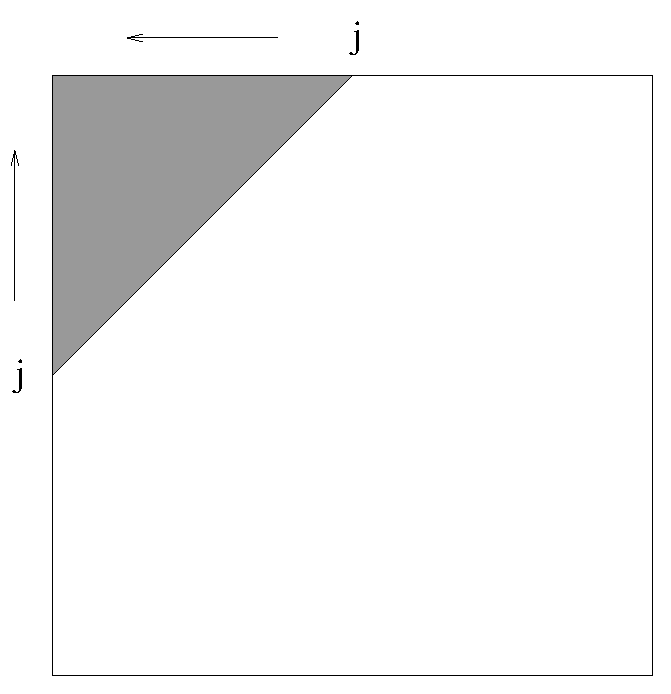
\includegraphics[width=5cm]{./zonal.eps}}
\caption{Área para retenção de coeficientes DCT.}\label{fig:zonal}
\end{center}
\end{figure}

\begin{enumerate}
\item[\textit{Dica}:] Multiplique elemento a elemento a DCT da imagem por uma máscara com 1's à esquerda e acima da diagonal \textsf{j}. Tal máscara pode ser gerada com os comandos:
\begin{verbatim}
A = zeros(size);
A(1:j,1:j) = fliplr(triu(ones(j)));
\end{verbatim}
\end{enumerate}

\item \textbf{Pergunta:} Explique o funcionamento da dica acima.

\item \textbf{Tarefa:} Avalie a imagem reconstruída em comparação com a original para os diferentes valores de \textsf{j} em função do MSE e do PSNR das imagens reconstruídas. Apresente uma tabela com esses valores.

\item \textbf{Pergunta:} Comente e explique os resultados presentes na tabela construída acima.

\end{enumerate}

\subsection{Compactação}

\begin{enumerate}

\item \textbf{Tarefa:} Agora, vamos processar a imagem em blocos de $8\times 8$ pixeis . 

\begin{enumerate}
\item Repita os itens 12.2.1 a 12.2.5, com \textsf{j} entre 1 e 8.
\end{enumerate}

\item \textbf{Tarefa:} Faça os histogramas dos valores dos coeficientes retidos, compare-os com os histogramas dos valores dos pixeis das imagens. Calcule as entropias correspondentes.

\item \textbf{Pergunta:} O que você conclui?

\end{enumerate}
\end{document}

